% Options for packages loaded elsewhere
\PassOptionsToPackage{unicode}{hyperref}
\PassOptionsToPackage{hyphens}{url}
%
\documentclass[
]{article}
\usepackage{lmodern}
\usepackage{amssymb,amsmath}
\usepackage{ifxetex,ifluatex}
\ifnum 0\ifxetex 1\fi\ifluatex 1\fi=0 % if pdftex
  \usepackage[T1]{fontenc}
  \usepackage[utf8]{inputenc}
  \usepackage{textcomp} % provide euro and other symbols
\else % if luatex or xetex
  \usepackage{unicode-math}
  \defaultfontfeatures{Scale=MatchLowercase}
  \defaultfontfeatures[\rmfamily]{Ligatures=TeX,Scale=1}
\fi
% Use upquote if available, for straight quotes in verbatim environments
\IfFileExists{upquote.sty}{\usepackage{upquote}}{}
\IfFileExists{microtype.sty}{% use microtype if available
  \usepackage[]{microtype}
  \UseMicrotypeSet[protrusion]{basicmath} % disable protrusion for tt fonts
}{}
\makeatletter
\@ifundefined{KOMAClassName}{% if non-KOMA class
  \IfFileExists{parskip.sty}{%
    \usepackage{parskip}
  }{% else
    \setlength{\parindent}{0pt}
    \setlength{\parskip}{6pt plus 2pt minus 1pt}}
}{% if KOMA class
  \KOMAoptions{parskip=half}}
\makeatother
\usepackage{xcolor}
\IfFileExists{xurl.sty}{\usepackage{xurl}}{} % add URL line breaks if available
\IfFileExists{bookmark.sty}{\usepackage{bookmark}}{\usepackage{hyperref}}
\hypersetup{
  pdftitle={HRD test},
  pdfauthor={Jun Kang},
  hidelinks,
  pdfcreator={LaTeX via pandoc}}
\urlstyle{same} % disable monospaced font for URLs
\usepackage[margin=1in]{geometry}
\usepackage{graphicx,grffile}
\makeatletter
\def\maxwidth{\ifdim\Gin@nat@width>\linewidth\linewidth\else\Gin@nat@width\fi}
\def\maxheight{\ifdim\Gin@nat@height>\textheight\textheight\else\Gin@nat@height\fi}
\makeatother
% Scale images if necessary, so that they will not overflow the page
% margins by default, and it is still possible to overwrite the defaults
% using explicit options in \includegraphics[width, height, ...]{}
\setkeys{Gin}{width=\maxwidth,height=\maxheight,keepaspectratio}
% Set default figure placement to htbp
\makeatletter
\def\fps@figure{htbp}
\makeatother
\setlength{\emergencystretch}{3em} % prevent overfull lines
\providecommand{\tightlist}{%
  \setlength{\itemsep}{0pt}\setlength{\parskip}{0pt}}
\setcounter{secnumdepth}{-\maxdimen} % remove section numbering

\title{HRD test}
\author{Jun Kang}
\date{2021 8 6}

\begin{document}
\maketitle

\hypertarget{myriad}{%
\subsection{Myriad}\label{myriad}}

{[}Myriad refers this
article{]}\url{https://clincancerres.aacrjournals.org/content/22/15/3764}

cut-off: 42

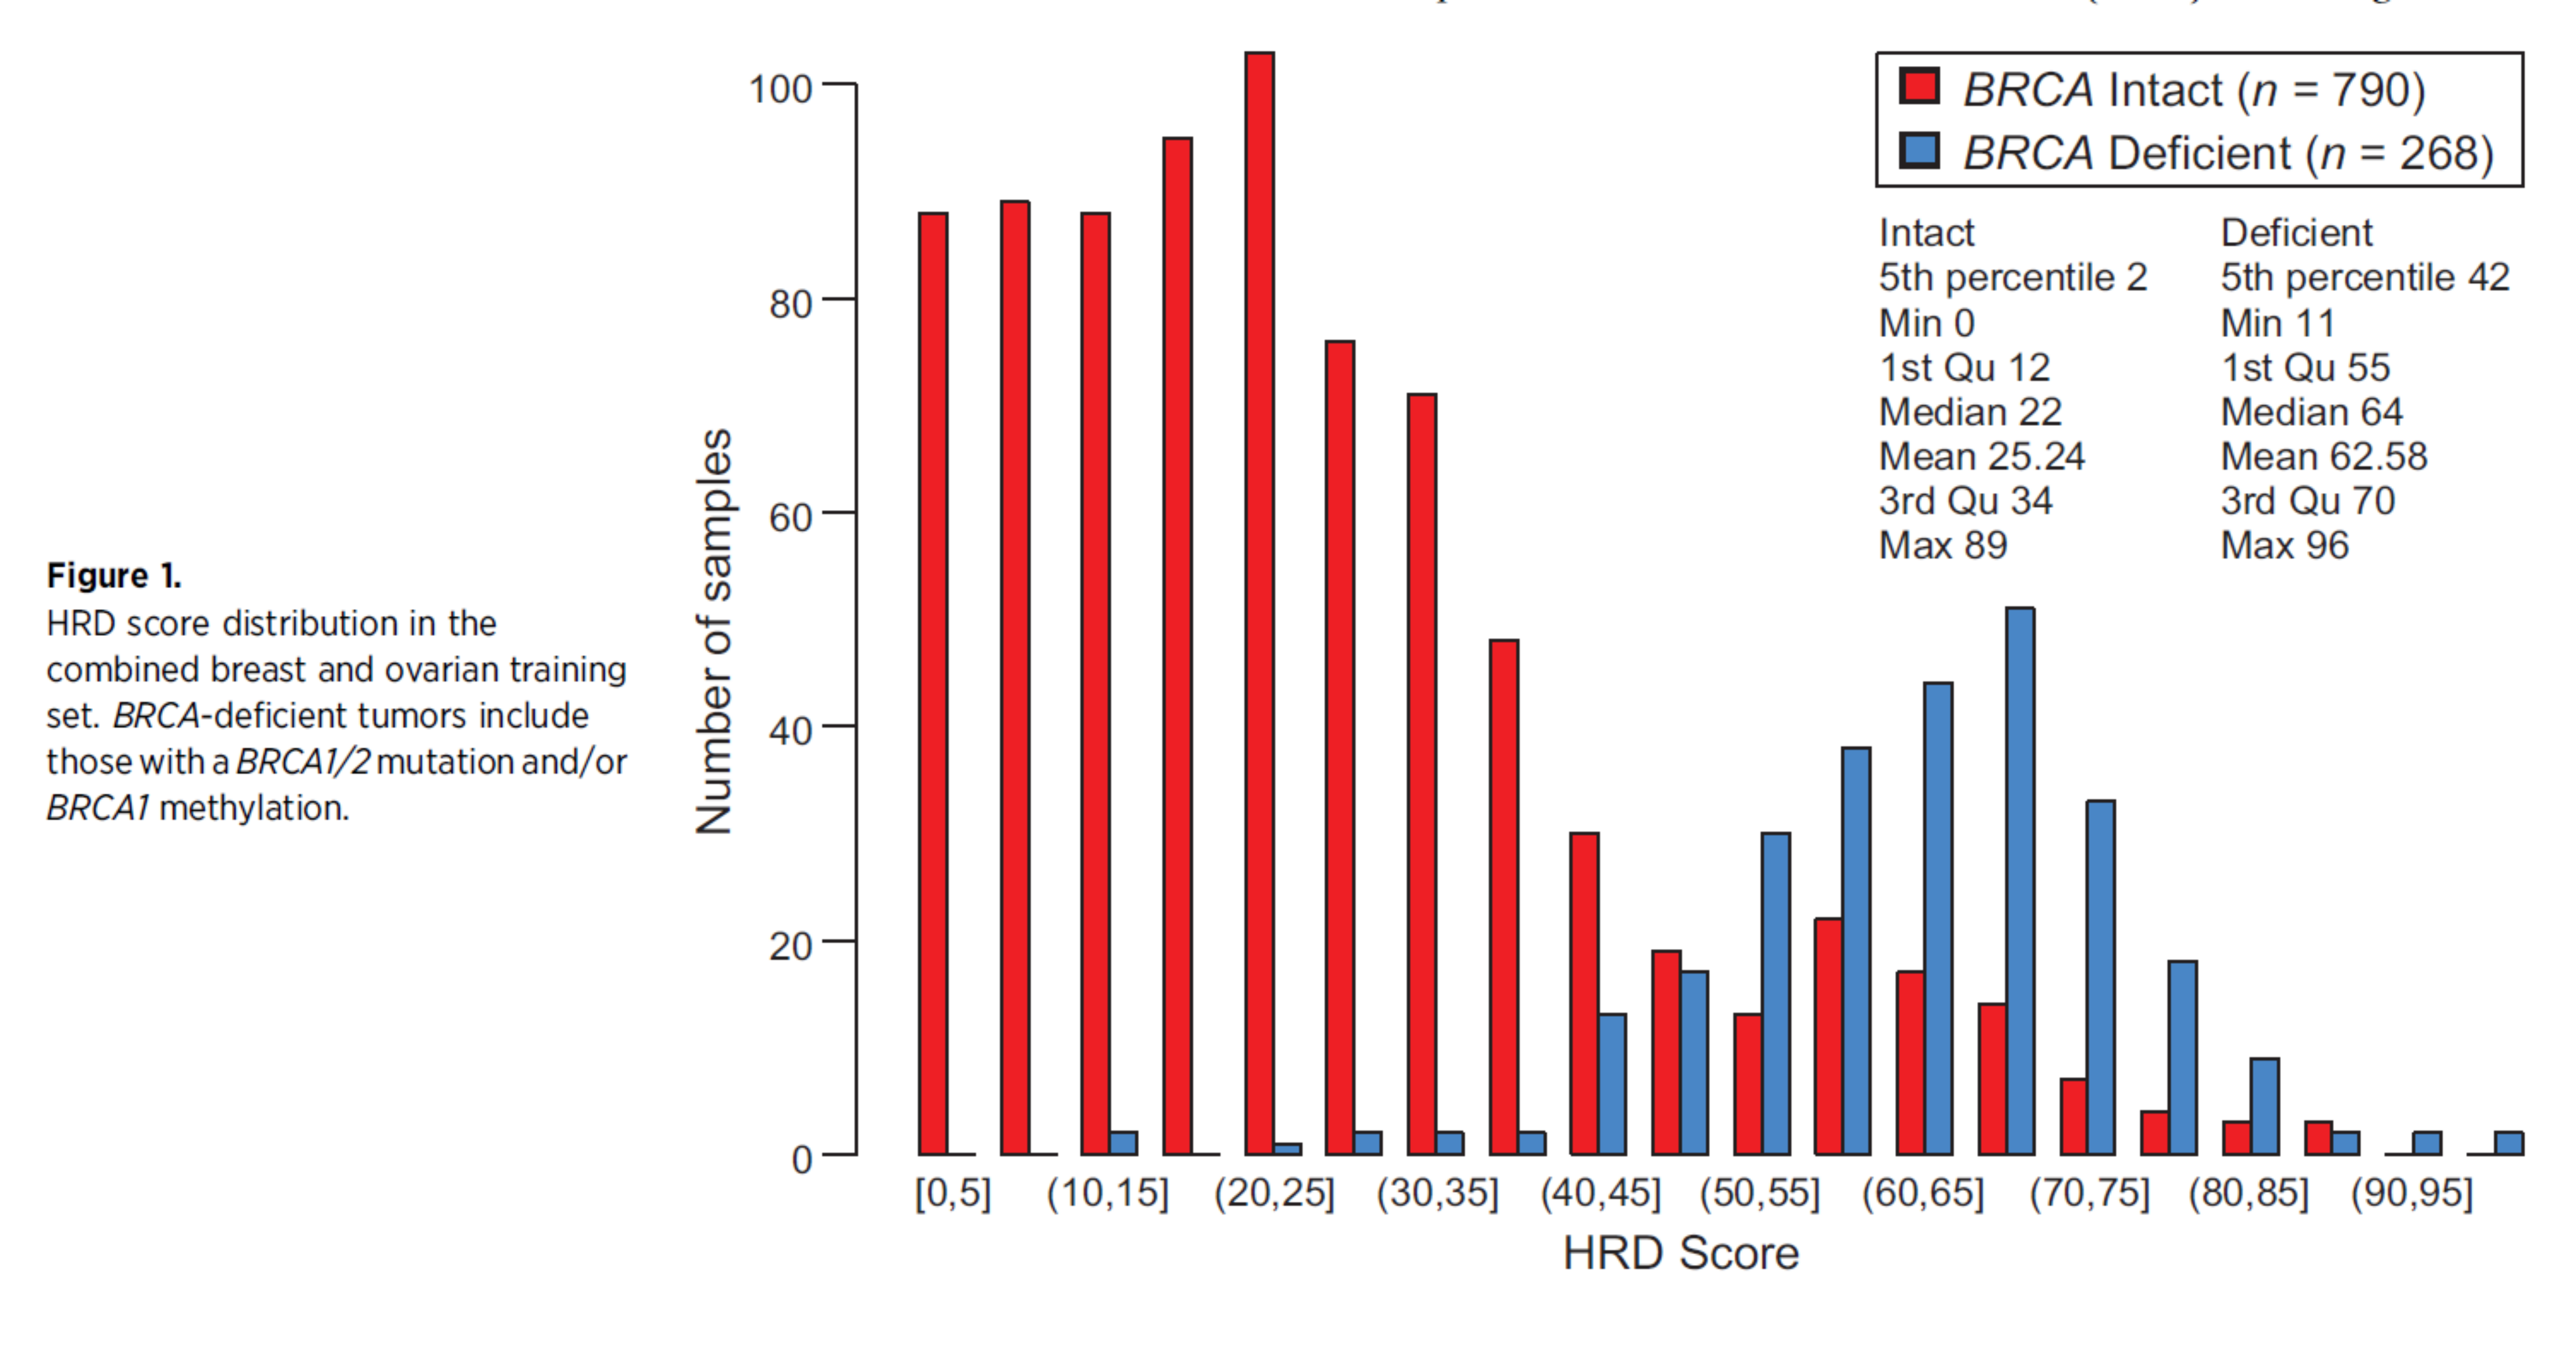
\includegraphics{img/telli.png}

\pagebreak

{[}Previous weighted
model{]}\url{https://breast-cancer-research.biomedcentral.com/articles/10.1186/s13058-014-0475-x\#additional-information}

HRD‐model=0.11xHRD‐LOH+0.25xHRD‐TAI+0.12xHRD‐LST

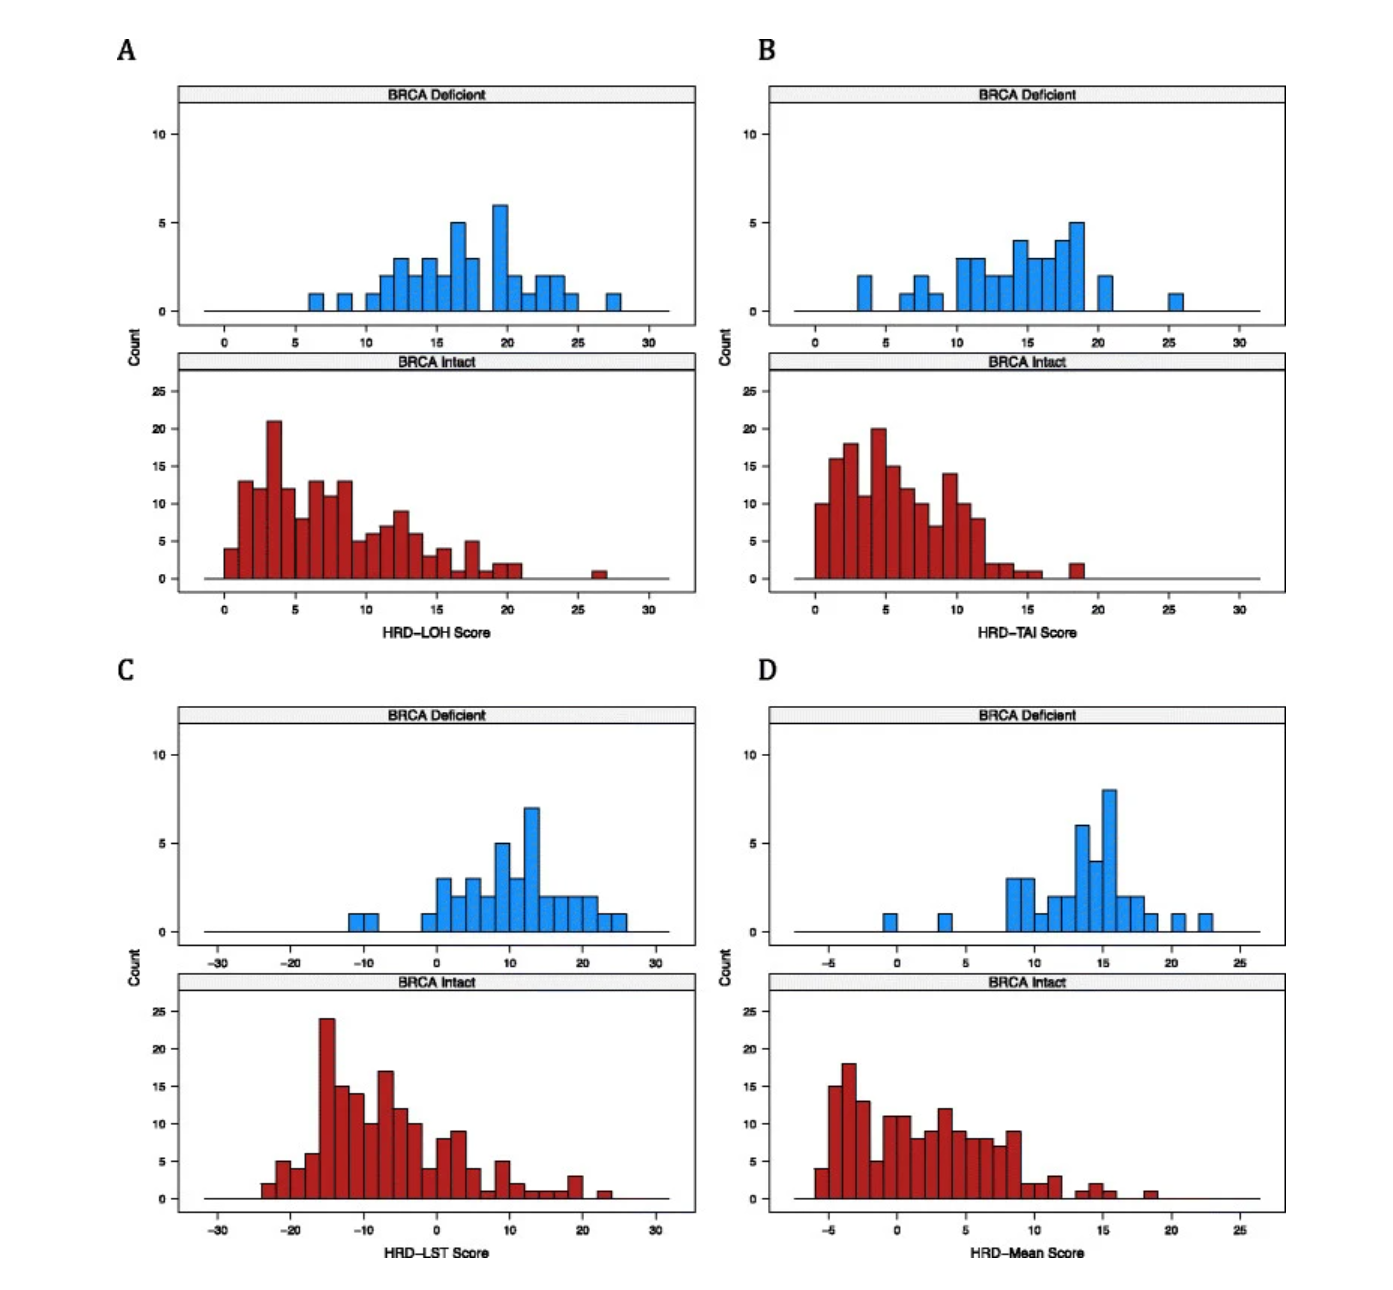
\includegraphics{img/Timms.png}

\pagebreak

\hypertarget{scarhrd}{%
\subsection{scarHRD}\label{scarhrd}}

{[}scarHRD Github{]}\url{https://github.com/sztup/scarHRD} {[}scarHRD
article{]}\url{https://www.nature.com/articles/s41523-018-0066-6}

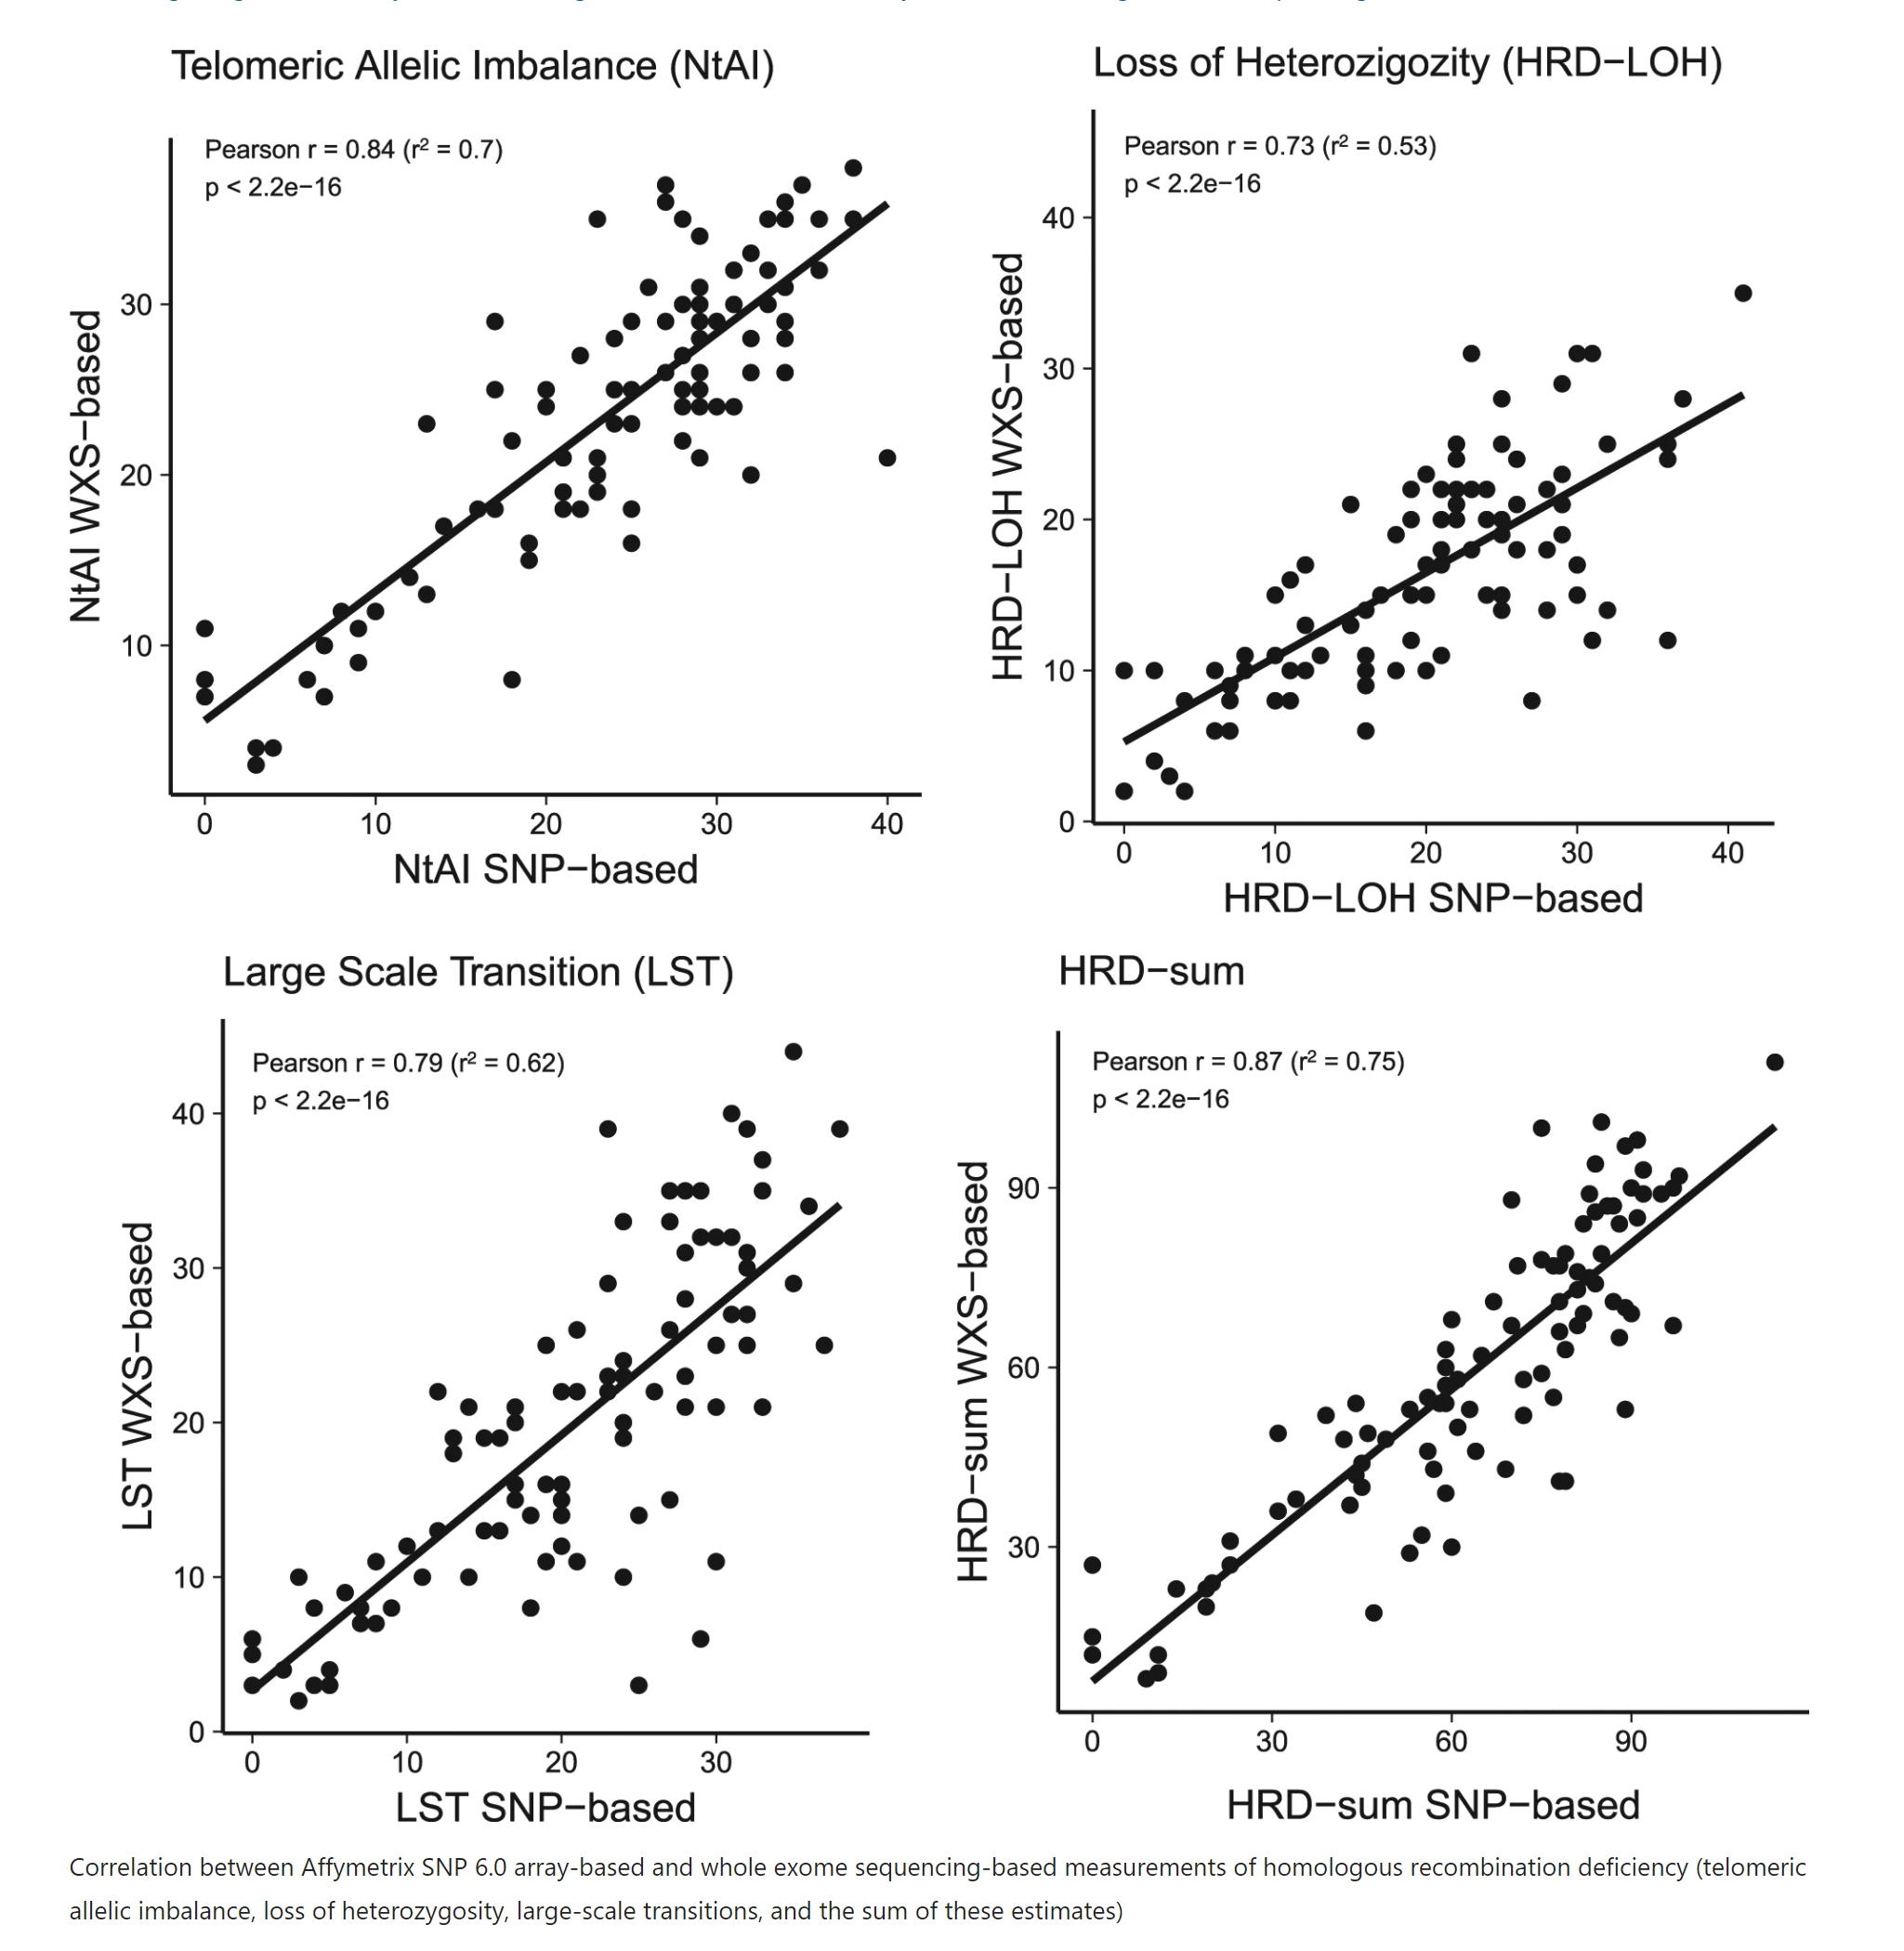
\includegraphics{img/scarHRD.png}

N.J.B., A.C.E., and Zo.S are listed as co-inventors on a patent on
telomeric allelic imbalance, which is owned by Children's Hospital
Boston and licensed to Myriad Genetics. The remaining authors declare no
competing interests.

\pagebreak

\hypertarget{hrdtools}{%
\subsection{HRDtools}\label{hrdtools}}

{[}HRDtools Github{]}\url{https://github.com/eyzhao/hrdtools}
{[}HRDtools
article{]}\url{https://clincancerres.aacrjournals.org/content/23/24/7521.long}

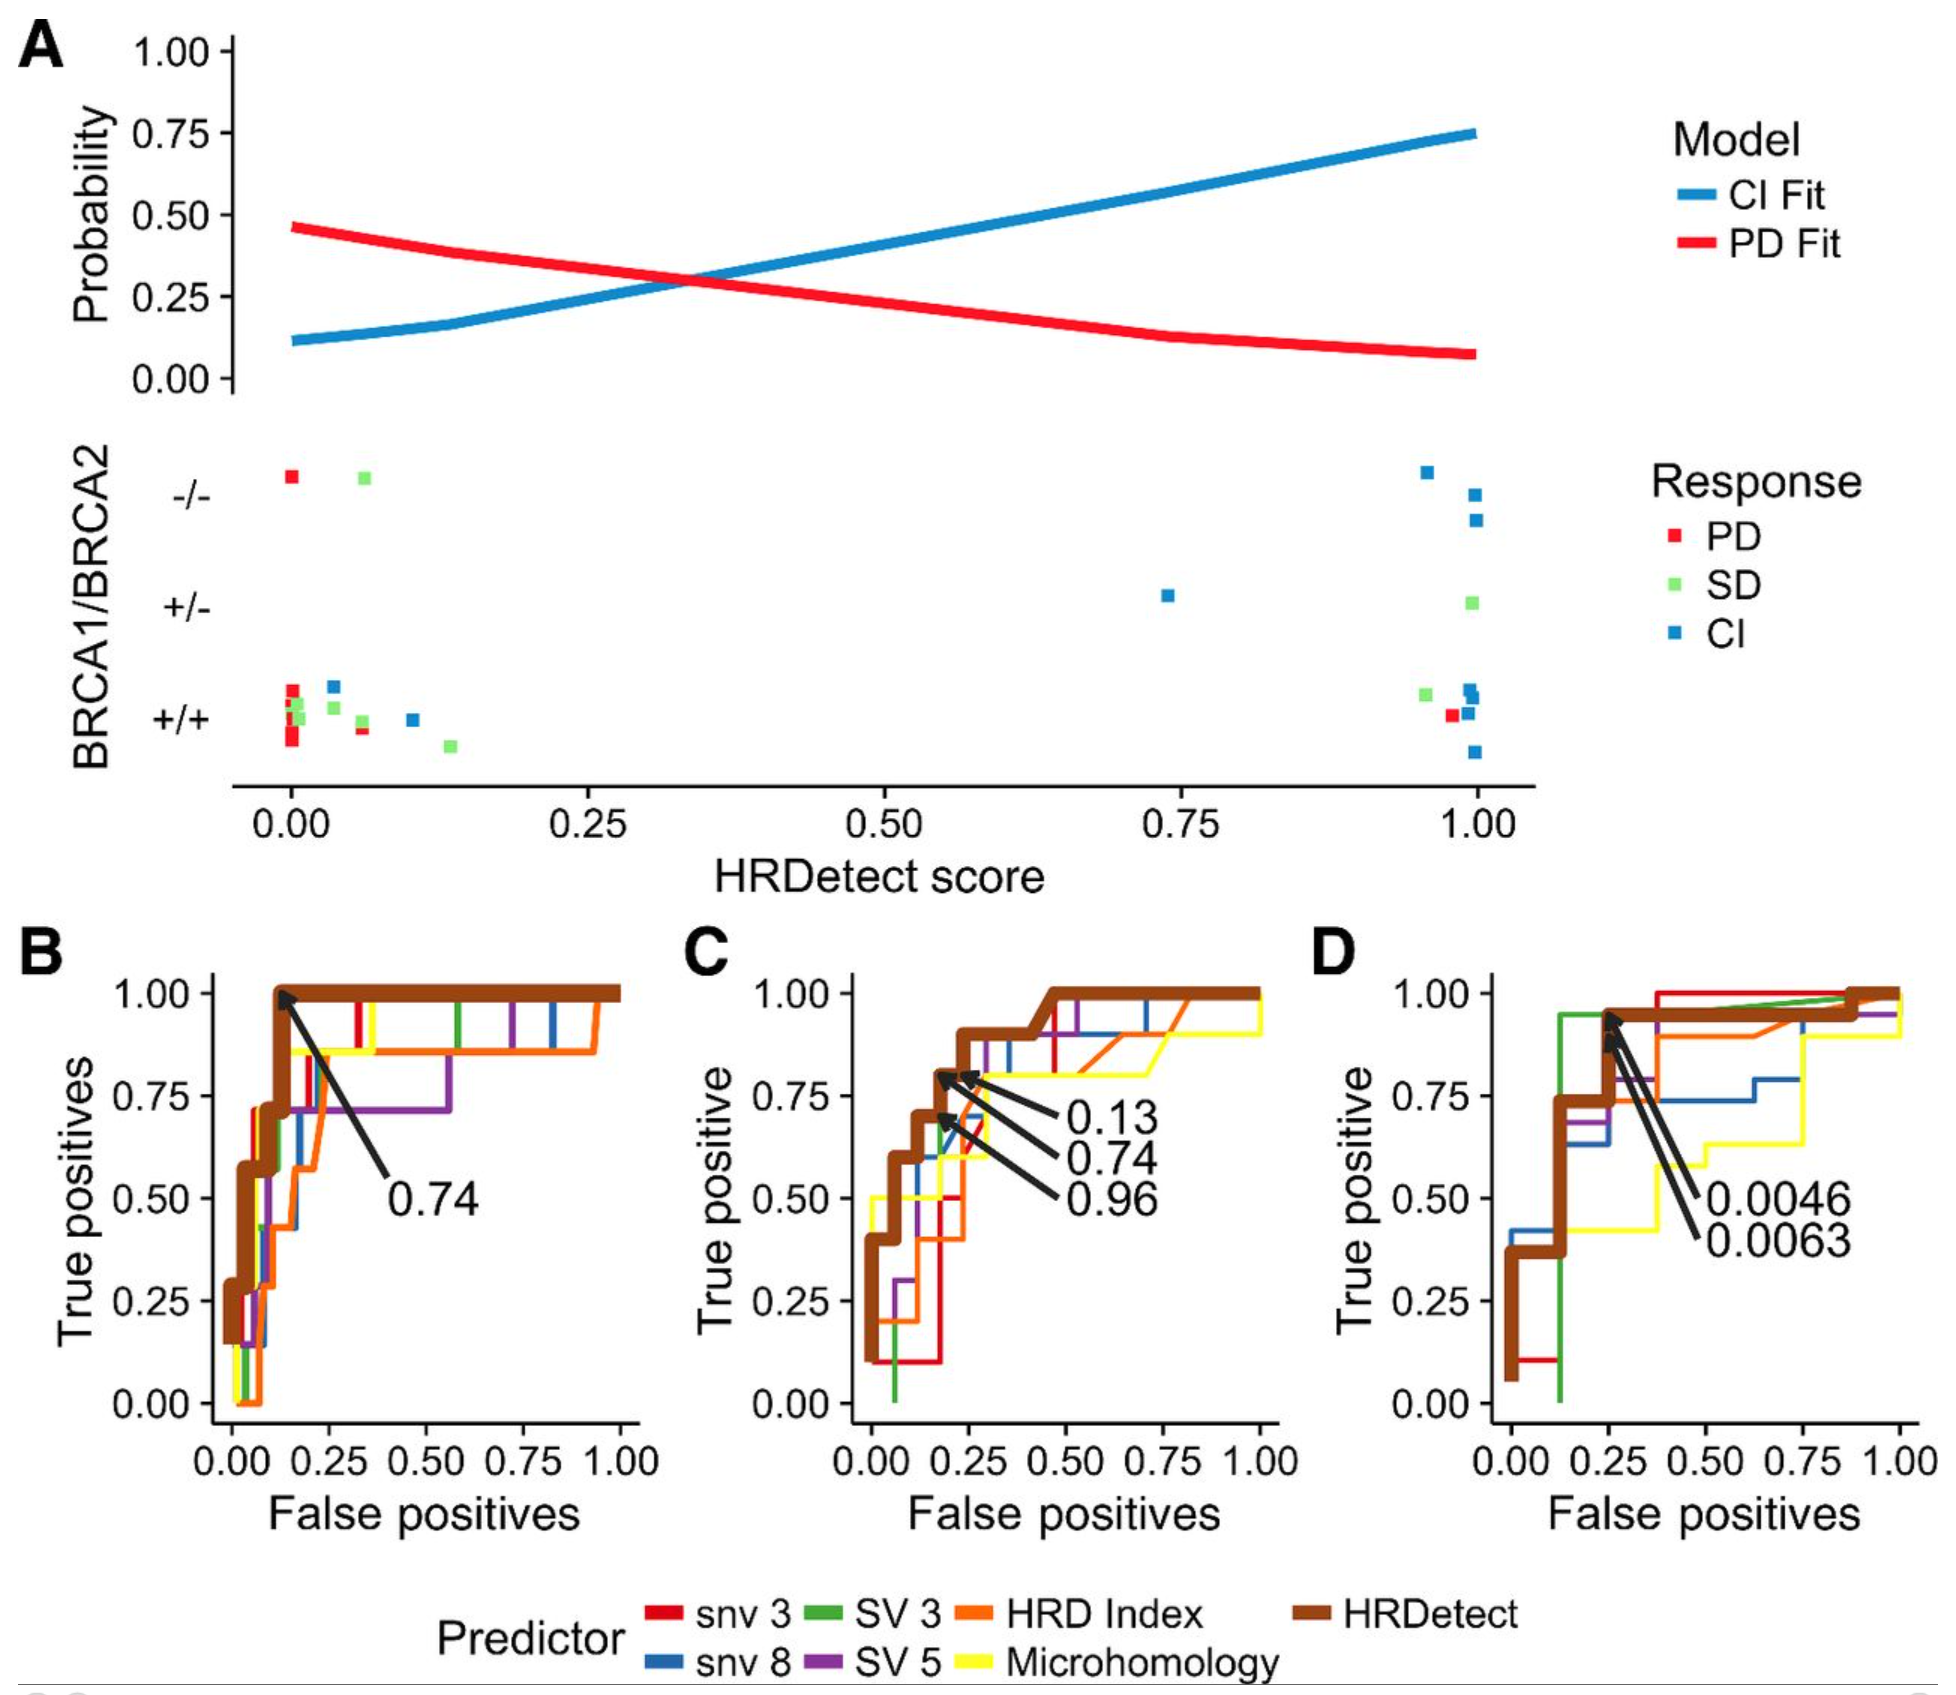
\includegraphics{img/HRDtools.png}

K.A. Gelmon reports receiving speakers bureau honoraria from Astra
Zeneca and Pfizer. S. Young reports receiving speakers bureau honoraria
from and is a consultant/advisory board member for Astra-Zeneca. No
potential conflicts of interest were disclosed by the other authors.

\pagebreak

\hypertarget{remarks}{%
\subsection{Remarks}\label{remarks}}

\begin{itemize}
\tightlist
\item
  Myriad and scarHRD might be similar.
\item
  Myriad program seems not to be publicaly opened.
\item
  scarHRD might be a good option for research purpose.
\end{itemize}

\end{document}
